\documentclass[11pt]{report}

\usepackage{geometry}
 \geometry{
 a4paper,
 total={210mm,297mm},
 left=25mm,
 right=25mm,
 top=30mm,
 bottom=25mm,
 headsep=7mm}

\interfootnotelinepenalty=10000

\usepackage{graphicx}
\usepackage{titlesec}
\usepackage{todonotes}
\usepackage{float}
\usepackage{hyperref}
\graphicspath{ {images/} }

\setcounter{secnumdepth}{4}


\begin{document}

	\begin{titlepage}
		\centering
		
\includegraphics{logo.png}\par\vspace{1cm}
		{\scshape\LARGE Politecnico di Milano \par}
		\vspace{1cm}
		{\scshape\Large Software Engineering 2\par}
		\vspace{1.5cm}
		{\huge\bfseries Requirements Analysis and Specifications Document\par}
		\vspace{2cm}
		{\Large\itshape Pietro Melzi, Alessandro Pina, Salvadore Matteo\par}

		\vfill

		% Bottom of the page
		{\large AA 2017-2018\par}
	\end{titlepage}

	\tableofcontents{}

	\chapter{INTRODUCTION}
	\label{ch:INTRODUCTION}
	
		\section{Purpose}
		\label{sect:Purpose}
			This document provides a baseline for the project planning of Travlendar+, the system we want to develop. It analyses the environment in which the system is intended to be used and contains information about the offered functions.
\newline
\newline
Travlendar+ is a service based on mobile application and web application that helps people to organize daily appointments and travels between them. The application wants to be a useful tool that can be used both in work time and in free time. In Travlendar+ the user simply has to create an event; the application will organize the travel in order to reach the location in the best way and will add the new event within the daily schedule. The user can modify the schedule with any feasible combination of added events and can specify different types of preferences on travel means, so the system can plan the trip according to personal needs.
\newline
\newline
People currently use different services, provided by calendar and maps applications, in order to organize meetings and events. Travlendar+ includes all the helpful functionalities you need to plan the day in the same application.

			
		\section{Scope}
		\label{sect:Scope}
			\subsection{Goals}
Travlendar+ is a service based on a mobile application and a web application.
\newline
\newline
The user simply has to create events and insert them into his schedule; the application will then organize travels in order to reach locations in the best way, correctly inserting them within the daily schedule and notifying eventual overlappings. \newline
The user can modify the schedule with any feasible combination of added events and can specify different types of preferences on travel means, so the system can plan the trip according to his personal needs.
\newline
\newline
The main functionality of the system is to control the user's daily flow of events, helping him optimizing his time and making sure that all his preferences and constraints are respected.
The principal goal of Travlendar+ is to save time, both in the construction of the schedule and in the traveling between events.
\newline
\newline

\underline{Visitor} should be able to:
\begin{description}
\item [[G1]] sign up into the system;
\end{description}

\noindent\underline{User} should be able to:
\begin{description}
\item[[G2]] log into the system;
\item[[G3]] create event specifying location, date, starting and ending time;
\item[[G4]] obtain the best path according to his preferences and the list of eventual alternative paths to reach a location;
\item[[G5]] change the selected path with an alternative path; 
\item[[G6]] obtain a daily schedule that allows to attend to every event in program;
\item[[G7]] apply constraints on travel means;
	\begin{description}
	\item[[G7.1]] related to the length of travel;
	\item[[G7.2]] related to the period of day;
	\end{description}
\item[[G8]] deactivate one or more travel means;
\item[[G9]] select combinations of transportation means that minimize carbon footprint;
\item[[G10]] reserve time for lunch or break events;
\item[[G11]] arrange trips;
	\begin{description}
	\item[[G11.1]] buy needed tickets;
	\item[[G11.2]] find available sharing vehicle.
	\end{description}
\end{description}

			\subsection{Domain properties}

\begin{itemize}
\item[D1] username must be unique;
\item[D2] every event is related to a location;
\item[D3] events must happen in an existing place;
\item[D4] events cannot be in the past;
\item[D5] starting time is always specified;
\item[D6] ending time is not mandatory;
\item[D7] a person can travel only on one travel mean at once; 
\item[D8] allowed travel means are cars, trains, metro, on foot, trams, bicycles, taxis, car sharing, bike sharing;
\item[D9] every travel is programmed with a combination of one or more travel means;
\item[D10] a person can be only in one place at once;
\item[D11] all travel means are related to information about average carbon footprints; 
\item[D12] flexible timeslots can have a daily or periodical validity;
\item[D13] every flexible timeslot has a minimum amount of time that must be reserved;
\item[D14] to use a public transport a ticket is required; 
\item[D15] a ticket may have a daily validity or a different periodicity; 
\item[D16] user can own day/week/season passes;
\item[D17] to use a sharing vehicle a payment is required;
\item[D18] a sharing vehicle must be parked in an allowed position.
\end{itemize}

			
		\section{Definitions, Acronyms, Abbreviations}
		\label{sect:Definitions, Acronyms, Abbreviations}
			\subsection{Definitions}
	\begin{itemize}
	\item Arrange trip: the system provides to the user all information about a travel. If the travel is related to one or more public travel means, the system helps the user to organize it. It is indicated if the user already holds a valid ticket for a certain travel or if he has to buy a required one. Purchase of a ticket is handled on the transport services' sites. Trip and travel are synonymous.
	\item Best path: it is the preferred travel option proposed to reach the event location among the feasible paths, according to a parameter specified by the user. Best path can be chosen according to one of these features: length, cost or environmental sustainability. Best path is the path taken into account and showed in the daily schedule; the user can substitute it with an alternative feasible path. 
	\item Break event: it is an optional event whose starting and ending time are flexible. The user can define this kind of event when he wants to reserve a certain amount of time in the schedule and he doesn't need to specify a starting time. For instance, a user could be able to specify that lunch must be possible every day between 11:30-
2:30, and it must be at least half an hour long, but the specific timing is flexible. The app would then be sure to reserve, if possible, at least 30 minutes for lunch each day.
	\item Constraint: it is a rule defined on travel means by the user. When the system calculates feasible paths each constraint must be taken into account: travel options opposed to constraints are ignored. A constraint can be associated to a type of event. There are different types of constraint: min/max distance allowed for a mean, interval of hour in which it is possible to take a mean and possibility to deactivate a mean. 
	\item Feasible path: a path that allows the user to reach a specified location before the event to attend starts and observes the constraints defined for that event.  
	\item Google maps API: a set of functions offered by Google Maps to decide  the path between two locations.
	\item Overlapping event: an event (or a part of it) that happen in the same time of another event, added previously in the schedule. Because the schedule must be feasible, an event is considered as "overlapping" also if only its related travel overlap an event present into the schedule.
	\item Periodicity: it is related to events that occur more than one time. It can be defined as weekly, monthly or in which days of week the event happen.
	\item Schedule: a daily plan with a set of events inserted by the user that allows him to travel and attend all the events. If an event overlap other events, it can not be inserted into the schedule. 
	\item Type of event: a set of rules (constraints) that is defined by the user and can be associated to a specific event several times.
	\item Transport service provider: a public or private company that controls and supplies the transport with a travel mean. 
	\item Travel: it is used to indicate the path that the user has to go across in order to reach a location. It can be made by several travel components.
	\item Travel component: each single path that can be done with a travel mean. It has a starting and ending time, a departure and arrival location and a length. The union of one or more travel components creates a travel.
	\end{itemize}
			\subsection{Acronyms}
	\begin{itemize}
	\item \textit{RASD}: Requirement Analysis and Specification Document;
	\item \textit{API}: Application Programming Interface.
	\end{itemize}
			\subsection{Abbreviations}
	\begin{itemize}
   	\item Gn: n-goal. 
   	\item Dn: n-domain assumption.
   	\item Rn: n-functional requirement. 
	\end{itemize}
			
		\section{Revision history}
		\label{sect:Revision history}
			2017/10/29 - Version 0.1.0 - First delivery of RASD.
			
		\section{Reference Documents}
		\label{sect:Documents}
			\begin{itemize}
\item Specification Document: “"Mandatory Project Assignments.pdf"”. 
\end{itemize}
			
		\section{Document Structure}
		\label{sect:Document Structure}
			This RASD is composed by six parts:
\begin{enumerate}
\item The first part of the document contains an introduction to the problem, where goals are identified and basic information is provided in order to better understand the rest of the document;
\item The second part of the document describes generally the system, identifying its boundaries and the actors involved in the life-cycle of the system. Boundaries are defined providing all the necessary assumptions: both the ones required in order to adapt to the user's specifications and the ones that will hold and from now on will be considered as true;
\item The third part of the document is composed by:
	\begin{itemize}
	\item a definition of functional and non functional specific requirements;
	\item a list of scenarios is provided: each of them describes a particular situation that the system might have to cope with;
	\item UML diagrams that model in detail the system behavior.
	\end{itemize}
\item The fourth part of the document contains the Alloy model of the system, including all the relevant 
details. It also provides a proof of consistency and an example of the world generated;
\item The fifth part of the document contains a report of the hours spent to write this document;
\item The sixth part of the document contains references to external documents used in this document.
\end{enumerate}

			
	\chapter{OVERALL DESCRIPTION}
	\label{ch:OVERALL DESCRIPTION}
	
		\section{Product perspective}
		\label{sect:Product perspective}
			\todo{TODO}
			\subsection{Class Diagram}
\noindent\makebox[\textwidth]{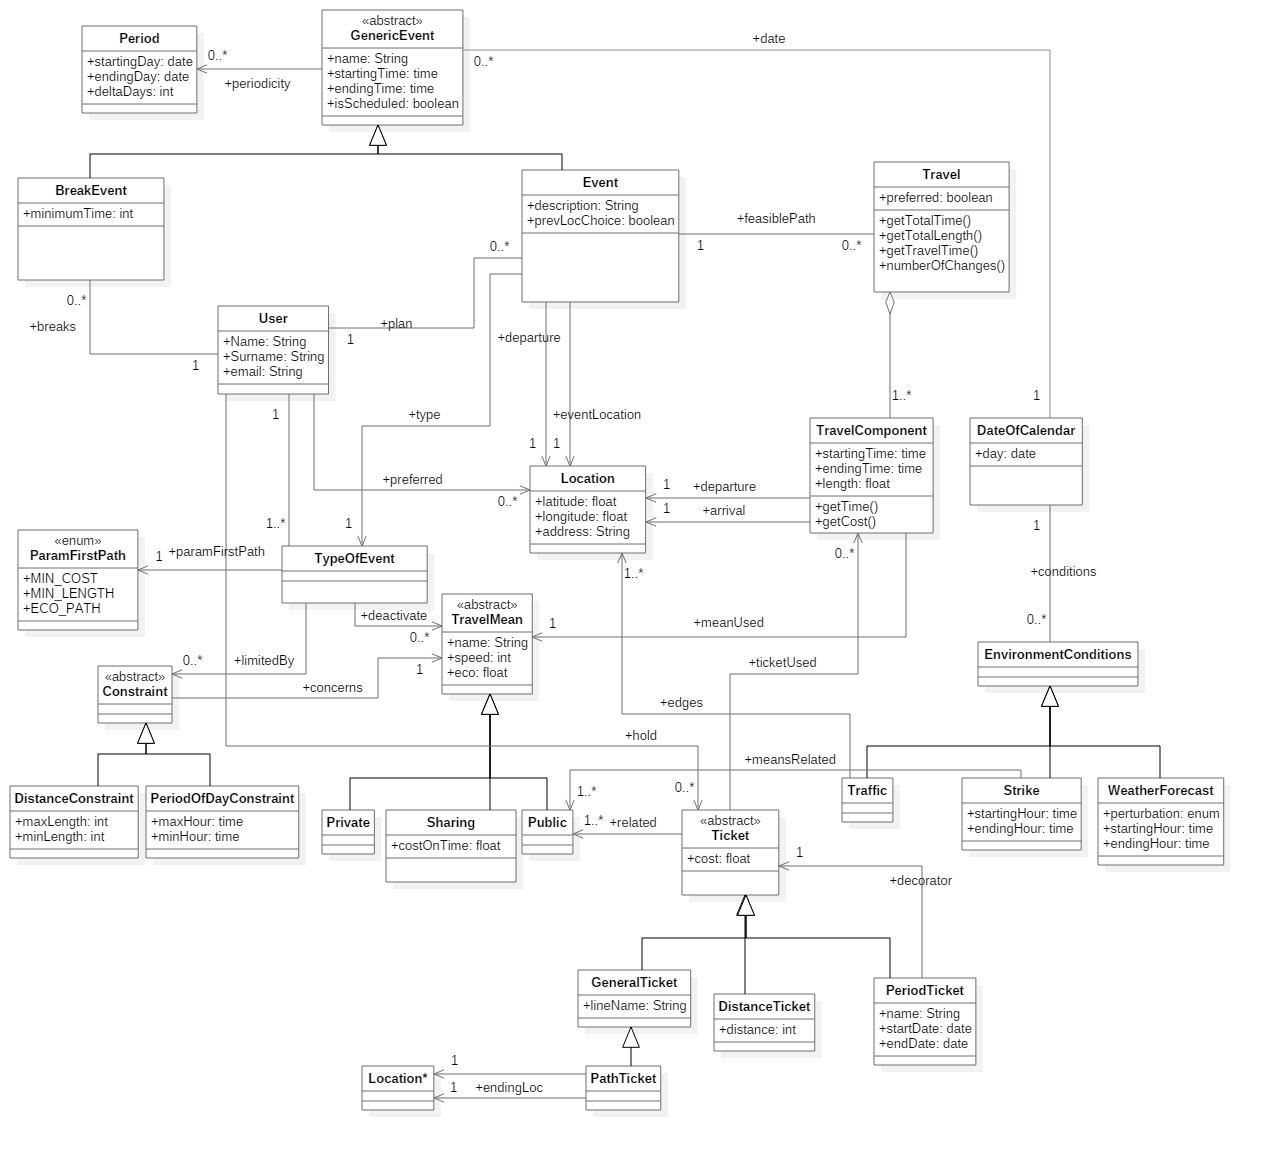
\includegraphics[width=\paperwidth,height=\paperheight,keepaspectratio]{class_diagram.jpg}}
\newline
An \textit{Event} is associated to one or more \textit{Travels}, a \textit{Travel} proposed requires the use of one or more \textit{Travel means}. The path of a \textit{Travel} that include different \textit{Travel Means} needs a structure where every \textit{Travel Component} (the path that can be performed with the same \textit{Travel Mean}), is memorized. Through a vector, an object of the \textit{Travel} class contains each \textit{Travel Component}.
\newline
\newline
\textit{Travel} class has the attribute \textit{preferred}: a Boolean value that identifies the path showed in the daily schedule for an inserted \textit{Event}. It must be checked that, for each \textit{Event}, only one \textit{Travel} is marked as preferred.
\newline
If a proposed path has different \textit{Travel Components}, information about time and length are provided by methods of the \textit{Travel} class that combine the values found in each related object of the \textit{Travel Component} class.
\newline
\newline
To represent \textit{Tickets} we use a hierarchy of classes: \textit{Distance Ticket} is used for tickets whose validity is indicated with a length, \textit{General Ticket} is used for particular tickets that allow the user to travel without constraints in a specified area, \textit{Path Ticket} is used when departure and arrival locations are indicated on the ticket. 
\newline
A \textit{Ticket} can be valid into specified dates or after the validation, for this reason the management of the time of validity is done with \textit{pattern Decorator}: it is used to specify the validity of an existing ticket.

		\section{Product functions}
		\label{sect:Product functions}
			\todo{TODO}
			A \textit{visitor} should be able to:
\begin{description}
\item[[G1]] sign up into the system:
	\begin{description}
	\item[[D1]] every inserted e-mail must be unique;
	\newline
	\item[[R1]] the system checks if the e-mail inserted is real;
	\item[[R2]] a user cannot sign up with the same e-mail twice.
	\end{description}
\end{description}

\noindent A \textit{user} should be able to:
\begin{description}
\item[[G2]] log into the system:
	\begin{description}
	\item[[D1]] every inserted e-mail must be unique;
	\newline
	\item[[R3]] the e-mail and password inserted must be correct;
	\item[[R4]] incorrect credentials prevent the user from logging in.
	\end{description}
\item[[G3]] create an event specifying its location, date, starting and ending time:
	\begin{description}
	\item[[D2]] every event is related to a location;
	\item[[D3]] an event must happen in an existing place;
	\item[[D4]] an event to attend cannot be in the past;
	\item[[D5]] the starting time of an event is always specified;
	\item[[D6]] the ending time of an event is not mandatory;
	\newline
	\item[[R5]] a user must specify all mandatory fields to add the new event;
	\item[[R6]] the system reserves the specified time-slot for the event;
	\item[[R7]] the system warns the user if the inserted event overlaps with an already existing one;
	\item[[R8]] if the ending time of an event is not specified, the systems considers as ending time the hour of departure for the successive event;
	\item[[R9]] when an event is inserted after an event without a specified ending time, the ending time  of the first event is anticipated as stated in [R8].
	\end{description}
\item[[G4]] obtain the best travel path (according to his preferences) and the list of eventual feasible alternatives to reach a location:
	\begin{description}
	\item[[D7]] a person can travel only on one travel mean at once; 
	\item[[D8]] allowed travel means are cars, trains, metro, on foot, trams, bicycles, taxis, car sharing, bike sharing;
	\item[[D9]] every travel is programmed with a combination of one or more travel means;
	\newline
	\item[[R10]] every travel path proposed must be feasible in the available time (the interval between two consecutive events);
	\item[[R11]] if the travel involves two or more travel means, the starting location of the first proposed travel path and the ending location of the last proposed travel path must coincide respectively with the starting location and the ending location of the whole planned travel;
	\item[[R12]] the system does not consider paths that violate constraints on travel means defined by the user;
	\item[[R13]] the system checks user preferences to decide which feasible travel path is the best;
	\item[[R14]] the system warns the user if it is not possible to arrive at an event location before its starting time;
	\item[[R15]] appropriate travel means must be suggested according to the type of event that they are related to; 
	\item[[R16]] if a strike occurs, the system will not consider travel means involved in it;
	\item[[R17]] if the weather forecasts rain or other adverse conditions, the system will not consider paths involving the bicycle.
	\end{description}
\item[[G5]] change the selected path with an alternative one:
	\begin{description}
	\item[[D7]] a person can travel only on one travel mean at once; 
	\item[[D8]] allowed travel means are cars, trains, metro, on foot, trams, bicycles, taxis, car sharing, bike sharing;
	\item[[D9]] every travel is programmed with a combination of one or more travel means;
	\newline
	\item[[R18]] the system must show to the user all possibilities to reach a location in according with the requirements of [[G4]];
	\item[[R19]] alternative feasible travel paths must not generate overlappings with other events of the schedule.
	\end{description}
\item[[G6]] obtain a daily schedule that allows him to attend every event in program:
	\begin{description}
	\item[[D10]] a person can be only in one place at once;
	\newline
	\item[[R20]] the combination of the travel paths proposed for the day must be feasible in the allotted time;
	\item[[R21]] if there are multiple events at the same time the system will propose in the schedule only the first event added.
	\item[[R22]] if the user forces into the schedule an event that overlaps with events already present in the schedule, these are removed from the schedule.
	\end{description}
\item[[G7]] apply constraints on travel means:
	\begin{description}
	\item[[D7]] a person can travel only on one travel mean at once; 
	\item[[D8]] allowed travel means are cars, trains, metro, on foot, trams, bicycles, taxis, car sharing, bike sharing;	
	\item[[D9]] every travel is programmed with a combination of one or more travel means;
	\newline
	\item[[R23]] the system requires minimum and maximum length allowed for a path to impose a constraint on a travel mean;
	\item[[R24]] the system requires an interval of time allowed to impose a constraint on a travel mean;
	\item[[R25]] the system does not consider solutions that violate constraints.
	\end{description}
\item[[G8]] deactivate one or more travel means:
	\begin{description}
	\item[[D7]] a person can travel only on one travel mean at once; 
	\item[[D8]] allowed travel means are cars, trains, metro, on foot, trams, bicycles, taxis, car sharing, bike sharing;	
	\item[[D9]] every travel is programmed with a combination of one or more travel means;
	\newline
	\item[[R26]] the system allows the user to specify one or more travel means that cannot be used;
	\item[[R27]] the system does not consider solutions that include deactivated travel means.
	\end{description}
\item[[G9]] select combinations of transportation means that minimize carbon footprint:
	\begin{description}
	\item[[D11]] every travel mean is related to information about its average carbon footprints;
	\newline
	\item[[R28]] for each travel path, the system estimates its carbon footprint produced.
	\end{description}
\item[[G10]] reserve time for lunch or break events:
	\begin{description}
	\item[[D12]] a flexible time-slot can have a daily or periodical validity;
	\item[[D13]] a flexible time-slot has a minimum amount of time that must be reserved;
	\newline
	\item[[R29]] the system allows the user to specify a flexible interval and a minimum amount of time to schedule a break;
	\item[[R30]] if there is enough time for a break, the system reserves it within the specified flexible interval;
	\item[[R31]] if there is not enough time into the flexible interval specified, a warning is thrown.
	\end{description}
\item[[G11.1]] arrange trips (buy needed tickets):
	\begin{description}
	\item[[D14]] a ticket is required to use a public transport;
	\item[[D15]] a ticket may have a daily validity or a different periodicity;
	\item[[D16]] a user can own day/week/season passes;
	\newline
	\item[[R32]] the system allows the user to specify all the ticket he already owns;
	\item[[R33]] the system shows to the user if he already holds a ticket for a proposed travel;
	\item[[R34]] the system allows the user to buy public transportation tickets according to proposed travels;
	\item[[R35]] the system provides information about time of departure and arrival of the proposed travels.
	\end{description}
\item[[G11.2]] arrange trips (find available sharing vehicles):
	\begin{description}
	\item[[D17]] a payment is required to use a sharing vehicle;
	\newline
	\item[[R36]] the system shows to the user where sharing vehicles are located;
	\item[[R37]] the system provides information about travel time with shared vehicles.
	\end{description}
\end{description}
			
		\section{User characteristics}
		\label{sect:User characteristics}
			\todo{TODO}
			
		\section{Assumptions, dependencies and constraints}
		\label{sect:Assumptions, dependencies and constraints}
			\todo{TODO}
			
	\chapter{SPECIFIC REQUIREMENTS}
	\label{ch:SPECIFIC REQUIREMENTS}
	
		\section{External Interface Requirements}
		\label{sect:External Interface Requirements}
			\subsection{User Interfaces}
\label{subsect:User Interfaces}
	\todo{TODO}
\subsection{Hardware Interfaces}
\label{subsect:Hardware Interfaces}
	\todo{TODO}
\subsection{Software Interfaces}
\label{subsect:Software Interfaces}
	\todo{TODO}
\subsection{Communication Interfaces}
\label{subsect:Communication Interfaces}
	\todo{TODO}
			
		\section{Functional Requirements}
		\label{sect:Functional Requirements}
			\subsection{Scenarios}
\label{subsect:Scenarios}
	\subsubsection{Scenario 1}
		Oscar is a businessman who travels a lot and he would like to organize his travels quickly and precisely. A friend advises him to try Travlendar+. Oscar enters the Travlendar+ website and loads the registration page by clicking on the 'signup' button, he fills all the mandatory fields and then he receives a confirmation email and he clicks on the confirmation link inside.
Then Oscar logs in and starts using Travlendar+.
	\subsubsection{Scenario 2}
		Nigel lives in Milan and tomorrow he’s going to have an appointment in Lecco, so he has to decide how to reach his appointment location; Nigel accesses the login page from his personal computer by using his browser, fills the username and password fields, clicks on the 'confirm' button and logs in. After he clicks on the dedicated button that adds a new event, he fills all the requested fields, setting the event type as 'work meeting' in order to obtain proper suggested travel means, then he confirms the event creation. On the next day, Nigel travels to Lecco, following the travel schedule proposed by his Travlendar+ app, reaching his appointment right on time.
	\subsubsection{Scenario 3}
		Jasper inserts an event into his Travlendar+ calendar, but the location inserted is too far away from his previous event, therefore a feasible path to reach the location of the next event is not available in the allotted time. Jasper is notified by a warning that he will not be able to reach his appointment in time.	
	\subsubsection{Scenario 4}
		Ophelia inserts a new event into his Travlendar+ calendar, but that event overlaps with another already existing event. Ophelia is notified by her app and the system asks Ophelia to choose which one of the overlapping events she wants to attend. She chooses the last event inserted, then she reads the travel means proposed to respect her new time schedule.
	\subsubsection{Scenario 5}
		Henrietta wants to personalize her Travlendar+ experience, so she clicks on the ‘menu’ icon and then the voice ‘preferences’. She selects her preferred travel means, she chooses to always obtain the fastest path and then, since she walks with a limp, she inserts a maximum walking distance of 500 meters. Before clicking on the 'confirm' button, she sees a polluting truck outside her window, so she decides to always follow travel paths that minimize her carbon footprint. She selects the relative option in her preferences. Finally she clicks on the ‘confirm’ button and she observes that her suggested travels have changed according to her new preferences.
	\subsubsection{Scenario 6}
		Arthur can\textsc{\char13}t concentrate on his work if he doesn't eat his lunch between 12.00 and 13.00. He also needs at least 25 minutes to consume a proper lunch.
For this reason Arthur inserts a flexible break event into his Travlendar+ calendar, in order to be sure that every day his app will reserve a time slot for his lunch.
A week later, Arthur inserts a new event whose travel overlaps with his flexible lunch event and his app notifies him. Arthur decides to ignore the warning, since he'll s going to eat during his travel.
	\subsubsection{Scenario 7}
		Gwendolyn looks at her Travlendar+ app and discovers that on the next day she has to travel first by train to Milan and then take a bike of MoBike’s sharing system in Milan. She clicks on the train travel slot in order to buy the proper ticket and the apps redirects her in the right Trenord’s online shop webpage. When she is about to buy the ticket she suddenly remembers that she has a weekly Trenord pass, therefore she cancels the transaction and, in order to avoid making the same mistake twice, she adds her pass information into her Travlendar+ app. The next day Gwendolyn takes the train to Milan and when she arrives she opens her Travlendar+ app in order to find the nearest bike of MoBike’s. Gwendoline arrives in time at her appointment.
	\subsubsection{Scenario 8}
		Harvey has to reach an appointment near his home next week. He adds an event in his Travlendar+ calendar. He observes that the app suggests him to use a bike to reach the location of this event. The day before his appointment the weather forecasts rain for the successive day, so Harvey is notified by his app that, due to the forecast, he should avoid taking the bike, suggesting instead to reach his appointment by car.
	\subsubsection{Scenario 9}
		Sara inserts an event in her Travlendar+ calendar, then she looks at the proposed travel path. Since she did not like the proposed travel, she clicks on the proposed path and selects another feasible alternative. The next day Sara travels according to the travel path she likes more.	
	
\subsection{Use case descriptions}
\label{subsect:Use case descriptions}

	\subsubsection{Registration}
		\begin{table}[H]
	\begin{center}
		\begin{tabular}{ | p{0.3\textwidth} | p{0.7\textwidth} | }
		\hline
		Participating actors & Generic visitor\\
		\hline
		Entry Condition & There are no entry conditions.\\
		\hline
		Event Flow & 
			\begin{enumerate}
				\item The visitor clicks on the “Register” button displayed onto the homepage;
				\item The visitor fills all the mandatory fields shown required by the system including his email, his password (twice) and a captcha;
				\item The visitor clicks on “Confirm” button;
				\item The visitor receives a confirmation email and clicks on the confirmation link;
				\item The system saves all user data inserted.
			\end{enumerate} \\
		\hline
		Exit Condition & The visitor’s registration is completed successfully, so the visitor is registered as an user of Travlendar+ and he can log in into the system as a registered user. \\
		\hline
		Exception & If:
				\begin{itemize}
   					\item The visitor insert an email already connected to an existing account;
   					\item Insert invalid infos into in some mandatory field;
   					\item Leave empty a mandatory field;
   				\end{itemize}
   		Then the system will request the visitor to complete/ revise all uncorrected field, highlighting them.
if the visitor doesn’t activate the account, after a month the activation link will expire and all user data will be deleted.\\ 
		\hline
		\end{tabular}
	\end{center}
	\caption{registration use-case}
\end{table}
		
	\subsubsection{Login}
		\begin{table}[H]
	\begin{center}
		\begin{tabular}{ | p{0.3\textwidth} | p{0.7\textwidth} | }
		\hline
		Participating actors & Unauthenticated User\\
		\hline
		Entry Condition & There are no entry conditions.\\
		\hline
		Event Flow & 
			\begin{enumerate}
				\item The visitor clicks on the 'Login' button displayed on the homepage;
				\item The visitor inserts the email and the password previously used for registration;
				\item The visitor clicks on 'Confirm' button;
				\item The system redirect the user to the main view of Travlendar+.
			\end{enumerate} \\
		\hline
		Exit Condition & The Visitor’s login is completed successfully, so the visitor can use all the Travlendar+ functions. \\
		\hline
		Exception & If:
				\begin{itemize}
   					\item The email inserted is not one of the emails previously used by an user to sign up;
   					\item The password inserted by the visitor is not the one associated with the email inserted;
   					\item At least one of the field is left empty;
   				\end{itemize}
   		Then the system will notify the visitor to complete/ revise all uncorrected field, highlighting them.\\ 
		\hline
		\end{tabular}
	\end{center}
\end{table}
		
	\subsubsection{View calendar}
		\begin{table}[H]
	\begin{center}
		\begin{tabular}{ | p{0.3\textwidth} | p{0.7\textwidth} | }
		\hline
		Participating actors & User\\
		\hline
		Entry Condition & The user must be logged in Travlendar+.\\
		\hline
		Event Flow & 
			\begin{enumerate}
				\item The user clicks on the calendar button;
				\item The system shows a calendar including all inserted events, and the travel paths related.
			\end{enumerate} \\
		\hline
		Exit Condition & The system let the user check his calendar. \\
		\hline
		Exception & There are no exceptions.\\ 
		\hline
		\end{tabular}
	\end{center}
\end{table}
		
	\subsubsection{Create event}
		\begin{table}[H]
	\begin{center}
		\begin{tabular}{ | p{0.3\textwidth} | p{0.7\textwidth} | }
		\hline
		Participating actors & User.\\
		\hline
		Entry Condition & The user must be registered and logged in Travlendar+\\
		\hline
		Event Flow & 
			\begin{enumerate}
				\item The user clicks on the dedicated button to add a new event;
				\item The user inserts all the info related to the event: date, starting time, ending time, location, name of the event, type of event (predefined or personalized), description, location starting from to reach the event's location;
				\item The user confirms the creation of the event;
				\item The system computes the best possible path according to the  user's preferences.
			\end{enumerate} \\
		\hline
		Exit Condition & The system redirects the user to the calendar and adds the travel time slot required to reach that event (comprehensive of travel description). \\
		\hline
		Exception & If the inserted event overlaps with one or more previously added events (the travel is also considered in the eventual overlap), then the user is notified with a warning message and the overlapping event is not considered in the user travel planning schedule (but it remains saved in the calendar). The user has to choose which one of the overlapped events does he want to attend.\\ 
		\hline
		\end{tabular}
	\end{center}
	\caption{Create event use-case}
\end{table}
		
	\subsubsection{Define preferences}
		\begin{table}[H]
	\begin{center}
		\begin{tabular}{ | p{0.3\textwidth} | p{0.7\textwidth} | }
		\hline
		Participating actors & User.\\
		\hline
		Entry Condition & The user must be registered and logged in Travlendar+.\\
		\hline
		Event Flow & 
			\begin{enumerate}
				\item The user opens the menu;
				\item The user selects the tab "Preferences";
				\item The user selects which type of event he wants to modify;
				\item The system shows a page containing fields to fill;
				\item The user defines his preferences by filling the fields on the page;
				\item The user clicks on the "Save" button.
			\end{enumerate} \\
		\hline
		Exit Condition & The user has selected his preferences, which have been saved correctly.\\
		\hline
		Exception & If the user exits the page without clicking the "Save" button, then the system will not save the preferences modified by the user.\\ 
		\hline
		\end{tabular}
	\end{center}
	\caption{Define preferences use-case}
\end{table}
		
	\subsubsection{Define flexible breaks}
		\begin{table}[H]
	\begin{center}
		\begin{tabular}{ | p{0.3\textwidth} | p{0.7\textwidth} | }
		\hline
		Participating actors & User.\\
		\hline
		Entry Condition & The user must be registered and logged in Travlendar+.\\
		\hline
		Event Flow & 
			\begin{enumerate}
				\item The user clicks on the dedicated button to add breaks into the schedule;
				\item The user inserts a flexible period of time (specifying starting and ending time) that will contain the break, along with the minimum amount of time that will be dedicated to it;
				\item The user also specifies the periodicity of the break (daily, weekly, monthly or until a specified date) or if it refers only to certain days of the week (until a specified date);
				\item The user presses the "Save" button. 
			\end{enumerate} \\
		\hline
		Exit Condition &  The system notifies the user that the info inserted about breaks are correctly saved.\\
		\hline
		Exception & If it is not possible to dedicate the allotted time to the breaks because of previously added events, than the system asks the user to change the length of the break.
\\ 
		\hline
		\end{tabular}
	\end{center}
	\caption{Define flexible breaks use-case}
\end{table}	
		
	\subsubsection{Arrange trips}
		\begin{table}[H]
	\begin{center}
		\begin{tabular}{ | p{0.3\textwidth} | p{0.7\textwidth} | }
		\hline
		Participating actors &  User, Transport service provider\\
		\hline
		Entry Condition & The user must be logged in Travlendar+.\\
		\hline
		Event Flow & 
			\begin{enumerate}
				\item The user opens his calendar
				\item The user clicks on the trip he want to arrange;
				\item The system shows all tickets to be buyed and the tickets already bought;
				\item The user clicks on the ticket he want to buy.
				\item The system redirect the user to the right website (of the right Transport service provider) in order to buy the tickets.
			\end{enumerate} \\
		\hline
		Exit Condition & The user has successfully arranged his travel. \\
		\hline
		Exception & There are no exceptions. \\ 
		\hline
		\end{tabular}
	\end{center}
	\caption{Arrange trips use-case}
\end{table}	
		
	\subsubsection{Locate the nearest sharing vehicle}
		\begin{table}[H]
	\begin{center}
		\begin{tabular}{ | p{0.3\textwidth} | p{0.7\textwidth} | }
		\hline
		Participating actors &  User, Transport service provider\\
		\hline
		Entry Condition & The user has opened the arrange trip tab and is about to travel.\\
		\hline
		Event Flow & 
			\begin{enumerate}
				\item The user open the map;
				\item The system shows in the map the nearest vehicle of car sharing according to the chosen path and the infos provided by the transport service provider;
			\end{enumerate} \\
		\hline
		Exit Condition & The user take and use the suggested vehicle. \\
		\hline
		Exception &
				\begin{itemize}
   					\item If no near vehicle is found the system re-compute another path and show it to the user;
   					\item if the user take a shared vehicle, but not the suggested one nothing happen, just as he has taken the suggested vehicle;
   				\end{itemize} \\ 
		\hline
		\end{tabular}
	\end{center}
\end{table}	
		
	\subsubsection{Add ticket possessed}
		\begin{table}[H]
	\begin{center}
		\begin{tabular}{ | p{0.3\textwidth} | p{0.7\textwidth} | }
		\hline
		Participating actors & User\\
		\hline
		Entry Condition & The user has opened the arrange trip tab.\\
		\hline
		Event Flow & 
			\begin{enumerate}
				\item The user selects the tab 'my tickets';
				\item The system show a page containing all the tickets and passes possessed by the user;
				\item The user clicks on the 'add ticket' button;
				\item The system show a page containing fields to fill;
				\item The user inserts info regarding the ticket/pass possessed;
				\item The user clicks on the 'save' button;
				\item The system adds the ticket/pass to those already present in the user account.
			\end{enumerate} \\
		\hline
		Exit Condition & The user has successfully inserted his ticket/pass in the system.\\
		\hline
		Exception & If the user exits the page without clicking the “save” button, then the system will not save the ticket added by the user.\\ 
		\hline
		\end{tabular}
	\end{center}
	\caption{Add ticket possessed use-case}
\end{table}	
	
	\subsubsection{Obtain feasible travel paths}
		\begin{table}[H]
	\begin{center}
		\begin{tabular}{ | p{0.3\textwidth} | p{0.7\textwidth} | }
		\hline
		Participating actors & User, Google Maps APIs.\\
		\hline
		Entry Condition & The user must be registered and logged in Travlendar+.\\
		\hline
		Event Flow & 
			\begin{enumerate}
				\item The user opens the "Calendar" tab;
				\item The user selects a day in the calendar;
				\item The system shows the proposed feasible paths (shown as travel events) between the events;
				\item If the user wants to select an alternative travel path, he can clicks on the travel event in order to choose among the proposed feasible alternatives.
			\end{enumerate} \\
		\hline
		Exit Condition & The user has seen the possible travel paths that can be used to reach his meetings.\\
		\hline
		Exception & If no feasible travel path exists between two events, the system shows a warning in the calendar.\\ 
		\hline
		\end{tabular}
	\end{center}
	\caption{Obtain feasible travel paths use-case}
\end{table}	
	
	\subsubsection{Create personalized event profiles}
		\begin{table}[H]
	\begin{center}
		\begin{tabular}{ | p{0.3\textwidth} | p{0.7\textwidth} | }
		\hline
		Participating actors & User.\\
		\hline
		Entry Condition & The user must be registered and logged in Travlendar+.\\
		\hline
		Event Flow & 
			\begin{enumerate}
				\item The user opens the preferences menu;
				\item The system shows the default type of event;
				\item The user selects the tab "Create personalized type of event";
				\item The system shows a page containing a text field to fill;
				\item The user inserts the name of the personalized type of event that he wants to create;
				\item The user inserts the constraints on travel means related to that type of event;
				\item The user clicks on the "Save" button;
				\item The system adds the new type of events to those already existing.

			\end{enumerate} \\
		\hline
		Exit Condition & The user has successfully added a new personalized type of event in the system.\\
		\hline
		Exception & If the user exits the page without clicking the "Save" button, then the system will not save the new personalized type of event created by the user.\\ 
		\hline
		\end{tabular}
	\end{center}
	\caption{Create personalized event profiles use-case}
\end{table}
	
	\subsubsection{Choose between overlapping events}
		\begin{table}[H]
	\begin{center}
		\begin{tabular}{ | p{0.3\textwidth} | p{0.7\textwidth} | }
		\hline
		Participating actors & User\\
		\hline
		Entry Condition & The user must be logged in Travlendar+, at least two events are overlapped.\\
		\hline
		Event Flow & 
			\begin{enumerate}
				\item The user clicks on the calendar button;
				\item The system shows a calendar including all inserted events, and the travel paths related, the overlapping events are displayed in a separate way in respect to the actual day schedule;
				\item The user drag the chosen overlapping event into his day schedule;
				\item The system remove the precedent event (in conflict) and put it into the overlapping event list;
				\item The system shows the new day schedule, with updated travel paths.
			\end{enumerate} \\
		\hline
		Exit Condition & The system let the user check his calendar. \\
		\hline
		Exception & There are no exceptions.\\ 
		\hline
		\end{tabular}
	\end{center}
	\caption{Choose between overlapping events use-case}
\end{table}
		
\subsection{Use case diagrams}
\label{subsect:Use case diagrams}
	\subsubsection{Visitors}
		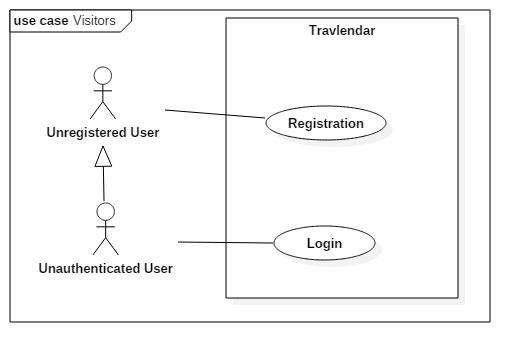
\includegraphics{Visitors.png}
	\subsubsection{User}
		\noindent\makebox[\textwidth]{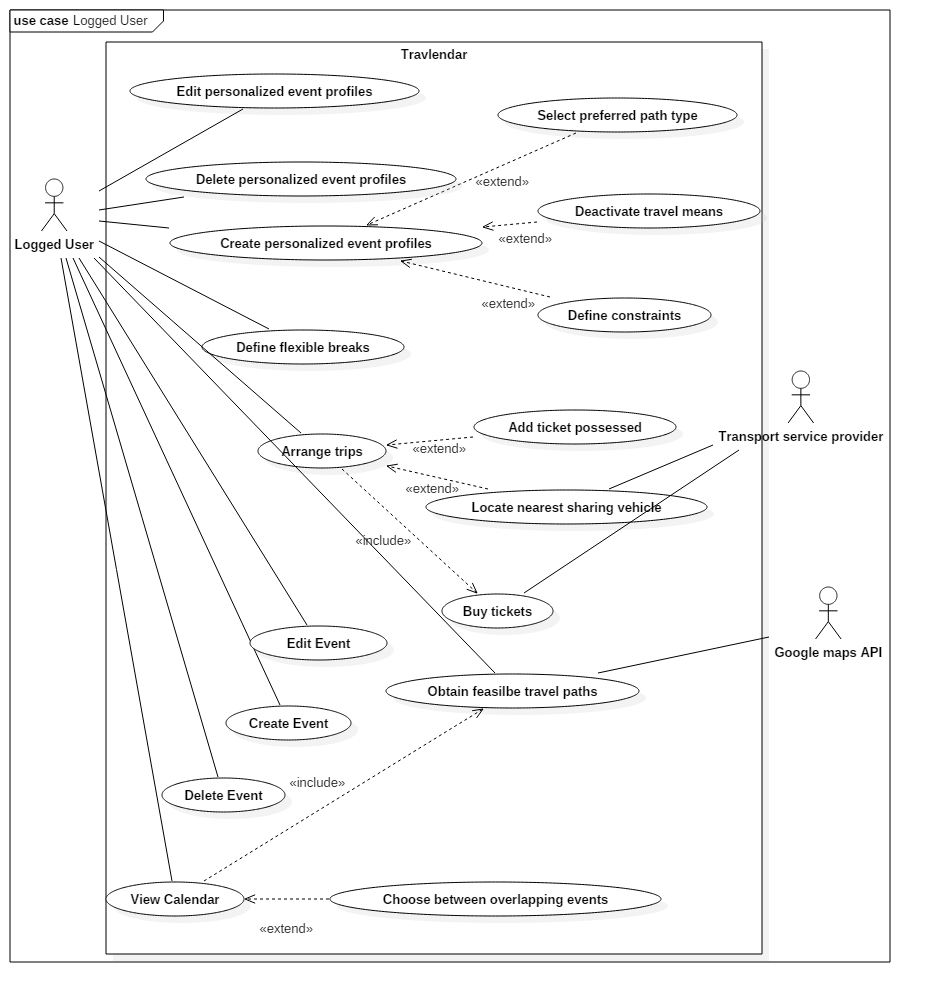
\includegraphics[width=\paperwidth,height=\paperheight,keepaspectratio]{LoggedUser.png}}
			
		\section{Performance Requirements}
		\label{sect:Performance Requirements}
			\todo{TODO}
			
		\section{Design Constraints}
		\label{sect:Design Constraints}
			\subsection{Standards compliance}
\label{subsect:Standards compliance}
	The system should produce a log containing all the action performed in the system, in order to able to perform a recovery in case of failures.
	\newline
	This recovery functionality is not implemented in this version of the system.
	\newline 
	Since the system memorize user's personal data it will have to respect privacy laws, in particular during the entire specification and development process we'll use as reference the General Data Protection Regulation (GDPR) (Regulation (EU) 2016/679), adopted in April 2016 by the European Union ( It becomes enforceable from 25 May 2018).
\subsection{Hardware limitations}
\label{subsect:Hardware limitations}
	In order to run on mobile devices, the application will need at least:
	\begin{itemize}
		\item 3G mobile internet connectivity;
		\item enough space in memory to install the application and store personal data;
		\item GPS module.
	\end{itemize}
	Since the application is primarily designed to be used on mobile phones while been away from home, low resolution and limited display size will be huge design constraints.
	\newline
	This also means that developing an effective user interface that can effectively show quickly and efficiently all the information necessary to the user will be a challenging task.
	\newline
	Also depending on the phone hardware, low processing power and small amount of memory are a matter of concern.

\subsection{Any other constraint}
\label{subsect:Any other constraint}
	Travlendar+ is dependent on external services to locate sharing vehicles, acquire tickets and produce travel paths. Because of this reason, it is critical to perform an update every time that one of these external functionalities changes, with the intent to avoid failures of the system.
	\newline
	Possible malfunctions of these external services should be accounted for during the development of Travlendar+, making sure that the system doesn't get hung up or crashes while trying to reach them.
			
		\section{Software System Attributes}
		\label{sect:Software System Attributes}
			\subsection{Reliability}
\label{subsect:Reliability}
	The reliability (Nb = 1 - Probability of failure) requested is related to many factors: the software developed must be stable and efficient in both server and client side, the user must satisfy the minimum requirement specifications specified in this document otherwise the reliability of the client app or the browser interface are not guaranteed; The reliability of the servers must be also taken into account and guaranteed by a proper maintenance .

\subsection{Availability}
\label{subsect:Availability}
	The system must offer an availability of 99\% (an overall 24/7 service). The remaining 1\% (at maximum) shall take into account the time spent for ordinary maintenance sessions. A backup server will be provided in order to maintain the availability of the service even after the main server failure.
\subsection{Security}
\label{subsect:Security}
	All user's data will be stored and encrypted using a proper hashing mechanism, even system administrators must not been able to access personal user's data. The GPS location of the users, detected by the mobile app, during the user's travels, is not to be memorized. All the connections established between users and server must use the
HTTPS protocol. Every communication between server and client will be encrypted.
\subsection{Maintainability}
\label{subsect:Maintainability}
	A version control system will be used in order to manage and organize all the different code revisions. In the development phase the entire source code will be properly documented and commented in order to ease the effort of possible future developers of understanding how the system has been designed and how it works. The documentation will also facilitate the system's maintenance. 
\subsection{Portability}
\label{subsect:Portability}
	The web application must support main browsers (such as Google Chrome, Mozilla Firefox, Microsoft Edge, Safari) latest version.\newline 
	The mobile application will be developed at first for Android architecture and then for iOS architecture.\newline
	The server-side of the application is written in Java, therefore it can be executed on any machine that runs a Java Virtual Machine.
			
	\chapter{FORMAL ANALYSIS USING ALLOY}
	\label{ch:FORMAL ANALYSIS USING ALLOY}
		\todo{TODO}
		
	\chapter{EFFORT SPENT}
	\label{ch:EFFORT SPENT}
		\todo{TODO}
		
	\chapter{REFERENCES}
	\label{ch:REFERENCES}
		\todo{TODO}

\end{document}
